%!TEX root = ../rules-working.tex
%LTeX: enabled=false

\begin{onecolumnfigure}[tp]

\begin{fitheight}{5.2\standardhexwidth}
\begin{tikzpicture}
    \setfiguresize{-3.5}{-2.6}{+3.5}{+2.6}
    \drawevenhexgrid{-3}{-2}{7}{5}
    \drawevenpositiongrid{-3}{-2}{7}{5}
\end{tikzpicture}
\end{fitheight}


\figurecaption{figure:map-location}{The hex grid defines a set of map locations at the center of each hex and at the center of each hex side. The map locations are shown here with dots.}

\vspace{\floatsep}

\silentlychangedin{1C}{1C-figures}{

\includegraphics[width=0.7\linewidth]{figures/figure-map-location.pdf}

}{

\begin{fitheight}{3.2\standardhexwidth}
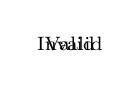
\begin{tikzpicture}
    \setfiguresize{-2.5}{-1.6}{+2.5}{+1.6}
    \drawevenhexgrid{-2}{-1}{5}{3}
    \drawaircraftcounter{-1.00}{+0.50}{90}{F-4}{A}{}
    \drawaircraftcounter{-1.50}{-0.75}{120}{F-4}{B}{}
    \drawaircraftcounter{+0.67}{+0.00}{0}{F-4}{C}{}
    \drawaircraftcounter{+1.50}{+0.75}{30}{F-4}{D}{}
    \miniathex{-2.00}{+0.00}{\node {\scriptsize Valid};}
    \miniathex{+2.00}{+0.00}{\node {\scriptsize Invalid};}
\end{tikzpicture}
\end{fitheight}


\figurecaption{figure:aircraft-map-location}{Map Location.}

}

\end{onecolumnfigure}
